\clearpage{\pagestyle{empty}\cleardoublepage}
\chapter{Design e Tecnologie}                %crea il capitolo
%%%%%%%%%%%%%%%%%%%%%%%%%%%%%%%%%%%%%%%%%imposta l'intestazione di pagina

Questo capitolo è dedicato alla presentazione del design e delle tecnologie utilizzate per la realizzazione del progetto.
Nelle apposite sezioni, saranno approfondite le caratteristiche di ciascuna tecnologia, in modo da offrire una panoramica completa sulle scelte implementative effettuate.


\section{Definizione dei Requisiti}
Vengono riportati di seguito i requisiti definiti in fase di progettazione, questi si dividono tra requisiti funzionali e requisiti non funzionali.
\subsection{Requisiti funzionali}
I requisiti funzionali definiscono il comportamento e le funzionalità del sistema \cite{requisiti}.
I requisiti individuati sono:
\begin{itemize}
    \item[RF1]: L'applicativo deve mostrare lo stato dell'inquinamento dell'aria in tempo reale;
    \item[RF2]: L'applicativo deve permettere all'utente di navigare su una mappa, compresa di funzionalità di ricerca e zoom;
    \item[RF3]: L'utente deve essere in grado di ascoltare una simulazione audio relativa all'inquinamento di qualsiasi parte del mondo, in qualsiasi data;
    \item[RF4]: Molteplici sonificazioni degli stessi dati devono risultare nella medesima traccia audio;
    \item[RF5]: Insieme allaf traccia audio sonificata deve essere mostrato un grafico progressivo raffigurante l'andamento dell'inquinamento;
    \item[RF6]: Il sistema deve funzionare su qualsiasi dispositivo e sistema operativo.
\end{itemize}

\subsection{Requisiti non funzionali}
I requisiti non funzionali definiscono le caratteristiche del sistema che non sono direttamente legate alle sue funzionalità.
Non sono solitamente richieste dal cliente e si rispecchiano nelle scelte laterali di progettazione e sviluppo \cite{requisiti}.
I requisiti non funzionali individuati sono:
\begin{itemize}
    \item[RNF1]: Il sistema deve essere semplice ed intuitivo da utilizzare;
    \item[RNF2]: L'applicativo deve astrattizzare qualsiasi riferimento alla sintesi audio e alla teoria musicale;
    \item[RNF3]: L'applicativo deve essere in grado di produrre una sonificazione in tempi relativamente brevi.
\end{itemize}



\section{Progettazione grafica}
In seguito alla definizione dei requisiti, sono passato alla fase di progettazione grafica.
\subsection{Mockup}

\begin{figure}[h]
    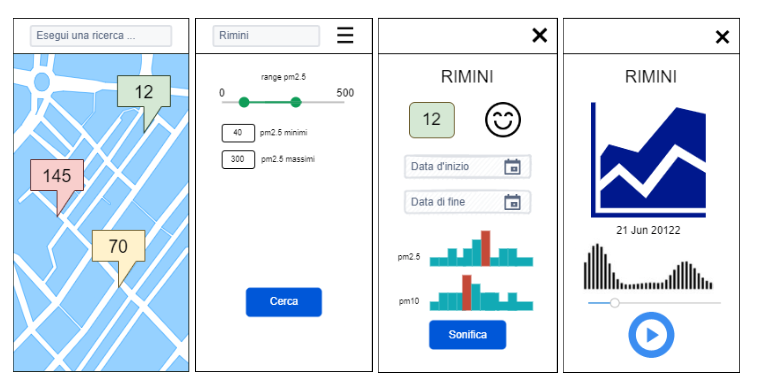
\includegraphics[width=\linewidth]{img/mockup.png}
    \caption{I mockup iniziali per la visualizzazione mobile}
    \label{fig:mockup}
\end{figure}

In Figura \ref{fig:mockup} sono riportati i mockup iniziali per la visualizzazione mobile dell'applicazione.
Per realizzare i mockups ho utilizzato la piattaforma online draw.io.
\begin{itemize}
    \item \textbf{Screen 1}: modella la prima view che viene mostrata, ogni pin rappresenta una stazione di rilevazione e il relativo indice di inquinamento in tempo reale. Al tap della casella di testo in alto viene aperta la view relativa a (Screen 2);
    \item \textbf{Screen 2}: In questa schermata l’utente può personalizzare la ricerca, mostrando solamente pin con inquinamento in un certo range, e spostare la camera sulla località selezionata;
    \item \textbf{Screen 3}: Al tap di un pin sulla mappa presente in (Screen 1), viene aperta la view relativa a (Screen 3). In questa schermata l’utente potrà selezionare l’intervallo di date il cui inquinamento rilevato verrà sonificato. Una volta selezionate le date, nei grafici sottostanti viene mostrata un’ anteprima dell’andamento delle rilevazioni nei giorni;
    \item \textbf{Screen 4}: Alla pressione del bottone Sonifica, viene mostrata la view relativa a (Screen 4), nella quale è presente un grafico che, tramite cambiamenti in tempo reale, accompagna la traccia audio generata a partire dai dati.
\end{itemize}

I mockup per la visualizzazione desktop non differiscono molto da quelli mobile, la mappa occupa l'intera pagina e le impostazioni per la sonificazione sono mostrate in un menu laterale a scomparsa (Figura \ref{fig:desktopmockup}).
\begin{figure}[H]
    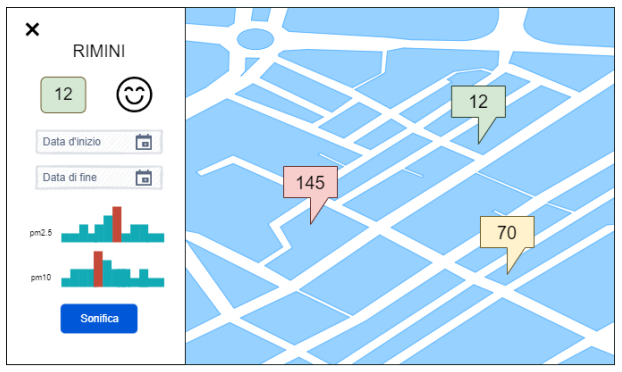
\includegraphics[width=\linewidth]{img/desktopmockup.PNG}
    \caption{I mockup iniziali per la visualizzazione desktop.}
    \label{fig:desktopmockup}
\end{figure}




%%%%%%%%%%%%%%%%%%%%%%%%%%%%%%%%%%%%
\section{Tecnologie web utilizzate}
L'idea di questo progetto nasce dalla necessità di fornire una rappresentazione della qualità dell'aria che respiriamo differente da quella solamente grafica.
Per questo fine ho deciso di sviluppare un'applicazione web: la risorsa informatica più facilmente accessibile ed utilizzabile.
A differenza di un'applicazione nativa, infatti, le webapp sono fruibili tramite browser da qualsiasi dispositivo connesso ad internet, senza bisogno di download o installazione \cite{appdiffs}.
Per comodità, ho suddiviso il programma in più parti: una parte di frontend, tramite la quale l'utente interagisce, e una parte di backend, che si occupa della sonificazione vera e propria.
In questa sezione verranno approfondite le tecnologie utilizzate per lo sviluppo del front end.

\subsection{HTML}
La pagina fruibile dall'utente presenta una struttura base HTML (Hyper Text Markup Language), un linguaggio per la formattazione di pagine web.
HTML è un linguaggio di pubblico dominio, la cui sintassi è stabilita dal World Wide Web Consortium (W3C): un'associazione non governativa che si occupa di diffondere l'accessibilità della rete e di standardizzare le tecnologie web.
La sintassi di HTML è composta da tag in cascata, i quali, letti dal browser, contengono le informazioni necessarie per l'impaginazione.

\subsection{CSS}
Il solo utilizzo di HTML non è sufficiente per ottenere un'interfaccia grafica gradevole e funzionale.
Per questo motivo ho utilizzato CSS (Cascading Style Sheet), un linguaggio utilizzato per definire lo stile di una pagina web, anch'esso reso standard da W3C da un insieme di regole.
CSS permette di attribuire stile grafico ai vari tag HTML, come ad esempio cambiare il colore di sfondo, la dimensione del testo e la posizione degli elementi.

\subsection{JavaScript}
Ho utilizzato Javascirpt per definire il comportamento della pagina in seguito alle interazioni dell'utente.
Javascript è un linguaggio di programmazione orientato ad eventi, interpretato durante l'esecuzione da un browser.
Javascript è comunemente utilizzato per introdurre effetti dinamici e funzionali chiamati eventi, invocabili dall'utente interagendo con la pagina HTML.
Ho scelto questo linguaggio per la sua semplicità nel gestire le richieste web, e per la sua ottima compatibilità con i vari browser.

\subsection{Jquery}
Spesso, collegare i tag HTML agli eventi definiti in Javasctipt, è un processo che, seppure non complicato, riempie il codice di debito tecnico.
Per questo ho delegato le interazioni tra le due tecnologie a Jquery: una libreria Javascript reperibile gratuitamente online.

\subsection{Bootstrap}
Bootstrap è una libreria di CSS disponibile gratuitamente, molto diffusa tra le applicazioni web.
Seppure questo framework si presti ottimalmente alla creazione di grafiche moderne e accattivanti, ho preferito limitarmi ad utilizzarlo per semplificare la gestione del layout della pagina, in particolare,
la posizione di elementi quali la mappa e il player video multimediale.

\subsection{Plotly}
Plotly è una libreria Javascript gratuita per la creazione di grafici.
Ho utilizzato questa libreria per creare i grafici che mostrano l'andamento dell'inquinamento nell'intervallo di tempo selezionato dall'utente.
Nonostante la libreria offra moltissimi stili di grafici, ho preferito utilizzare il grafico a barre, in quanto ritengo sia il più adatto per rappresentare questo tipo di dati.
Lo stile che ho deciso di applicare al grafico riprende i colori selezionati per lo standard AQI (visibili in tabella \ref{tab:aqi}). Ogni rilevazione viene colorata in base al livello di inquinamento.

\subsection{Leaflet - OpenStreetMap}
Ho utilizzato questi moduli per inserire una mappa interattiva all'interno della pagina web.
Leaflet è una libreria JavaScript open source per la gestione di mappe, facilmente estendibile e con una sintassi ad eventi simile a JQuery.
Per quanto riguarda invece l'aspetto della mappa ho applicato un layout vettoriale fornito da OpenStreetMap: un progetto open source sulla rappresentazione cartografica della superficie terrestre.
Tramite queste due componenti, l'utente può ingrandire la mappa e posizionare marker a proprio piacimento.
Siccome i colori utilizzati da EPA per l'AQI (tabella \ref{tab:aqi}) sono particolarmente chiari, ho applicato lo stile scuro, per aggiungere un contrasto maggiore.

\subsection{Esri Leaflet}
Al fine di permettere all'utente di eseguire ricerche per indirizzo e località, e reperire le informazioni di qualsiasi luogo alla pressione sulla mappa, ho utilizzato la libreria Esri Leaflet.
Esri Leaflet è una libreria JavaScript open source per la gestione dei dati geografici distribuita da Esri, un'azienda specializzata in questo campo.
Le funzionalità che ho utilizzato principalmente sono il geocoding e il reverse geocoding, ovvero la ricerca di coordinate geografiche a partire da un indirizzo e viceversa.

\subsection{AQIcn API}
Per ottenere i dati relativi alla qualità dell'aria da posizionare sulla mappa, ho utilizzato l'API di AQIcn.
Una API (applicaztion program interface), è un insieme di funzioni e procedure che, fungendo da interfaccia, permettono di interagire con un software esterno \cite{api}.
Questo servizio è stato messo a disposizione dal team del World Air Quality Index: un progetto no-profit che mira alla sensibilizzazione delle persone sulla tematica dell'inquinamento atmosferico.
AQIcn è un'implementazione di questo progetto, che fornisce agli sviluppatori, o ai soli interessati, dati trasparenti e aggiornati sulla qualità dell'aria in tempo reale.

\subsection{Weatherbit.io}
Purtroppo, al momento della progettazione e scelta delle tecnologie, l'API di AQIcn non metteva a disposizione una funzione per ottenere lo storico dei dati.
Per questo motivo, ho dovuto ricorrere ad una seconda API: Weatherbit.io.

\subsection{Javascript Fetch API}
Per rendere comunicanti la parte di frontend, la parte di backend e le varie API, ho utilizzato la funzioni Fetch messa a disposizione da javascript.
Tramite una chiamata Fetch, è possibile inviare una richiesta HTTP ad un server, e, se necessario, ricevere risposta.
Una chiamata a aquesta funzione permette di personalizzare la richiesta in base alle esigenze e al protocollo utilizzato; specificando l'URL di destinazione, modificando l'header e il body della richiesta, e gestendo la risposta.
Le chiamate a Fetch sono svolte in maniera asincrona; dove necessario ho utilizzato la caratteristica sintattica await per mantenere il flusso di esecuzione, aspettando il completamento della chiamata prima di proseguire.

\subsection{Python FastAPI}
Il software di backend che si occupa di gestire le richieste HTTP e fornire loro risposta è realizzato in Python.
Ho scelto questo linguaggio per la sua semplicità nella manipolazione di complesse strututre dati, e per l'enorme quantità di funzionalità matematiche offerte.
La libreriea utilizzata per elaborare le richieste di rete è FastAPI.
Tramite FastAPI è possibile creare un server web in maniera veloce, utilizzando parole chiave comuni nella sintassi di python.
Il software prodotto è una Restful API: un programma che utilizza il protocollo HTTP per ricevere e fornire dei dati \cite{api}.
Siccome il processo di sonificazione non è istantaneo, ogni richiesta viene gestita indipendentemente dalle altre, rendendo il server asincrono.




%%%%%%%%%%%%%%%%%%%%%%%%%%%%%%%%%%%%
\section{Tecnologie utilizzate per la sonificazione}

La software componente che esegue la sonificazione vera e propria è realizzata in Python in uno script differente da quello del server.
Il server, quando richiesto, esegue questo script passandogli come argomento tutti i dati necessari per produrre la traccia.
I dati inviati sono sotto forma di JSON, un formato standardizzato perticolarmente adatto all'interscambio di dati in rete.
I dati ricevuti dallo script di sonificazione sono: 
\begin{itemize}
    \item \textbf{data}: array di interi relativi alle varie rilevazioni;
    \item \textbf{days}: array di DateTimes, variabili rappresentanti l'orario e la giornata di ogni rilevazione;
    \item \textbf{index}: l'indice delle varie rilevazioni, può essere AQI, PM2.5 e PM10.
\end{itemize}
Questo programma svolge diversi compiti in successione, questi sono: ricevere i dati, creare le varie traccie, unirle in un'unico file wav, generare un'animazione in .gif, unire audio e video.

\subsection{Strategia di sonificazione}
Per sonificare i dati, ho utilizzato un approccio misto, sfruttando sia la sintesi audio che il design sonoro, approfonditi nel capitolo precedente.
Prima di progettare il sistema sonificativo, ho individuato le caratteristiche dei dati che volevo rappresentare:
le componenti di maggiore importanza sono l’andamento temporale dell'inquinamento e l'inquinamento residuo.
\subsubsection{L'andamento dell'inquinamento}
L'andamento temporale è rappresentato dalle varie rilevazioni nel tempo, siccome è un valore che tende a cambire rapidamente nel tempo, ha richiesto un approccio di sonificazione dinamico.
La scelta delle note utilizzate per rappresentare questo dato è molto semplice: più il valore dell'inquinamento è alto, più la nota è grave.
\subsubsection{L'inquinamento residuo}
L'inquinamento residuo consiste nel valore di rischio per la salute che si protrae nel tempo in seguito ad una giornata particolarmente inquinata.
A differenza della rilevazione AQI vera e propria, i cui valori possono variare drasticamente da un momento all'altro, l'accumulo di residuo si distingue in fasi di crescita e di diminuzione, in funzione a come si è comportato l'inquinamento nel corso della giornata \cite{residue}.
Per le fasi di crescita ho usato delle note veloci che si alzano di tonalità, mentre per la fase di diminuzione le stesse note sono ripetute con meno frequenza, e tendono ad abbassarsi nel tempo.
\subsubsection{Gestire il volume}
Un aspetto molto rilevante che ho attribuito a queste due traccie sta nella miscela dei loro volumi: più il valore dell'inquinamento tende ad alzarsi, più il suo volume si abbassa per lasciare spazio alla traccia dell'inquinamento residuo, che invece tende a crescere.
\subsubsection{L'applicazione della teoria musicale}
Per accentuare l'effetto della crescita e della diminuzione dell'inquinamento residuo, le note della traccia seguono una scala: più l'inquinamento è alto più le note sono acute.
Ho deciso di utilizzare una scala maggiore. Siccome le tonalità maggiori sono note per la loro positività, ho introdotto delle dissonanze in base al peggioramento della qualità dell'aria, volte a spezzare questa armonia.
Una dissonanza è una nota “fuori contesto” rispetto alla scala o all'accordo che si sta suonando; se inserita all'interno di una scala maggiore, sempre positiva e armoniosa, la dissonanza crea un effetto improvviso di tensione \cite{dissonance}.
Ho posto le dissonanze ad intervalli regolari nella scala in base al livello di inquinamento: più questo è alto, più le dissonanze sono frequenti e di maggior intensità.


\subsection{Design audio}
\subsubsection{I file MIDI}
Per quanto riguarda la parte di design audio, ho deciso di generare un file MIDI.
Il MIDI (Musical Instrument Digital Interface) è uno standard di comunicazione sviluppato agli inizi degli anni 80', è tutt'ora vastamente usato nel mondo della produzione musicale per la sua semplicità e la sua portabilità.
Tramite questo protocollo, è possibile comunicare gli stessi dati sia a software musicali che a dispositivi hardware, come tastiere e sintetizzatori, che li traducono in suoni \cite{midi}.
La creazione, modifica ed esportazione di tracciati MIDI è molto semplice in quanto non richiede alcuna conoscenza di linguaggi di programmazione e funzionamento del suono a livello hardware e software.
In aggiunta, la manipolazione della sequenza di note, è un processo incredibilmente più semplice e intuitivo rispetto alla modifica del segnale audio vero e proprio.
Una sequenza MIDI è una sequenza di eventi che si differenziano per la loro funzione; un evento ha un tempo di inizio, un tempo di fine, un canale e un valore.
Per misurare il tempo, i software musicali utilizzano vare metriche: battute di pentagramma, millisecondi, o tick MIDI.
Di default, un tick MIDI equivale a 1/960 di una battuta di pentagramma, il tempo è di 4/4 e la velocità è di 120 bpm \cite{midi}.
I principali eventi sono:
\begin{itemize}
    \item \textbf{Note On}: indica l'inizio di una nota, quando un tasto sulla tastiera viene premuto;
    \item \textbf{Note Off}: indica la fine di una nota, quando un tasto sulla tastiera viene rilasciato;
    \item \textbf{Control Change}: indica un cambiamento di stato, come ad esempio il cambio di tonalità di una nota mentre suona;
    \item \textbf{Program Change}: indica un cambio di strumento;
    \item \textbf{Meta Event}: indica un evento generale, può essere un messaggio di testo o un cambio di tempo.
\end{itemize}
Una sequenza MIDI può essere creata da uno strumento munito di tastiera, o da una Digital Audio Workstation: un software di produzione musicale; in particolare, queste ultime, presentano un'interfaccia sempre più incentrata sull'utilizzo di questo standard.
Lo strumento digitale più adatto alla composizione del MIDI è il piano roll: un editor che permette di visualizzare le note in un piano virtuale, mostrato in Figura \ref{fig:pianoroll}. 
Nel piano roll, ogni nota è rappresentata da una casella, la sua posizione orizzontale indica il tempo in cui inizia, mentre la sua posizione verticale indica la tonalità.
\begin{figure}[H]
    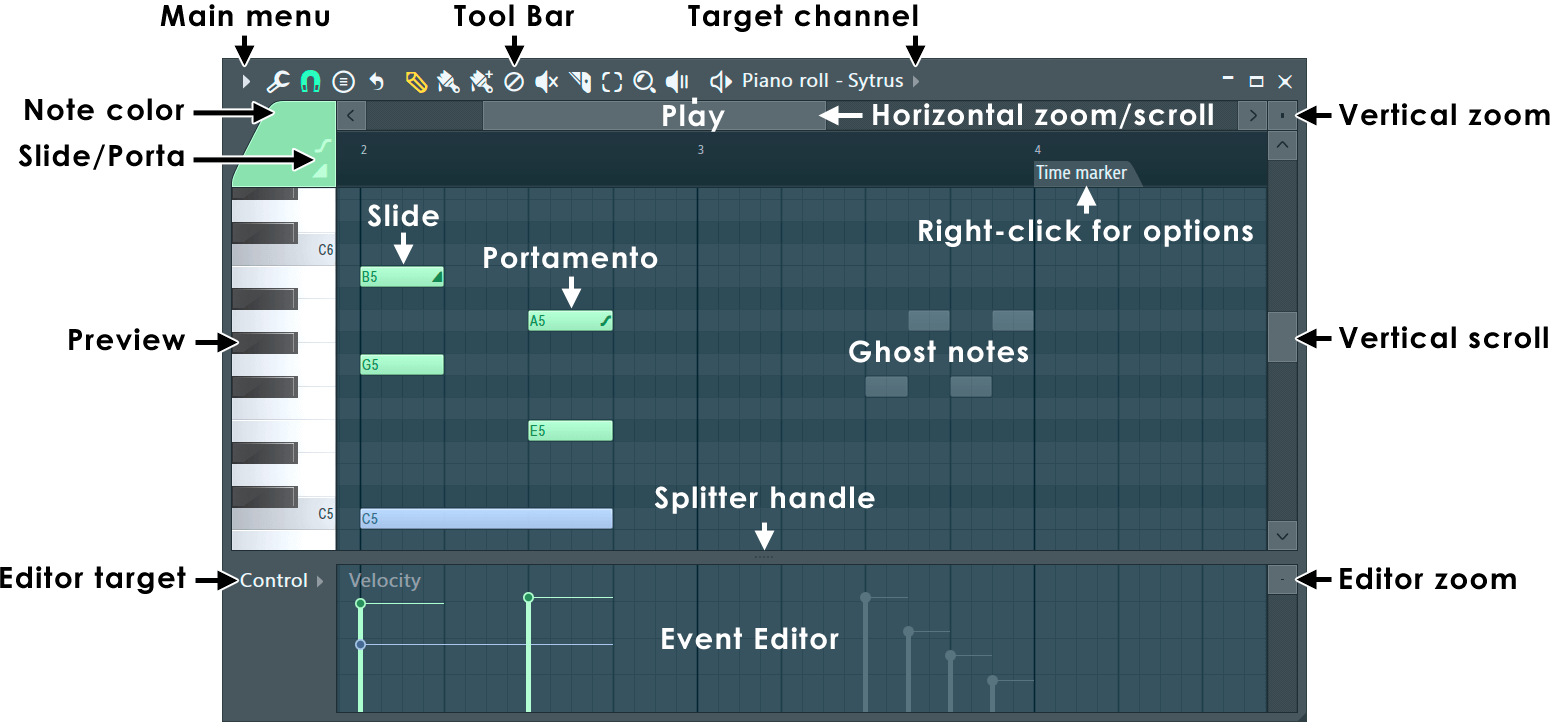
\includegraphics[width=\linewidth,scale=0.2]{img/pianoroll.png}
    \caption{Il piano roll di un software Digital Audio Workstation \cite{pianoroll_img}.}
    \label{fig:pianoroll}
\end{figure}
Lo standard MIDI, infine, comprende GeneralMidi: un'enumerazione di strumenti ed effetti audio.
Questa caratteristica mi ha permesso di concentrarmi solamente sulla scelta degli strumenti General MIDI e sulla generazione della sequenza di note, delegando la sintesi vera e propria ad un software terzo.
Per la creazione di file MIDI ho utilizzato MidiUtils, una libreria per Python che permette di creare un file MIDI specificandone i vari eventi.
Per la sintesi del file MIDI, invece, ho utilizzato Timidity++, un software open source che permette di sintetizzare un file MIDI in un file wav.
\subsubsection{Effetti audio VST3}
Per aggiungere spessore alle traccie midi sintetizzate, ho deciso di applicarvi degli effetti audio.
Scrivere effetti audio con risultati di qualità è un processo complesso, che richiede una conoscenza approfondita della propagazione del suono.
Per questo motivo, ho importato nel programma degli effetti audio sviluppati da professionisti.
La tecnologia che ho scelto è VST3 (Virtual Studio Technology 3), un formato che standardizza l'interfaccia tra il plugin e il software che lo utilizza.
Il formato VST è stato introdotto da Steinberg nel 1996 nel suo software Digital Audio Workstation Cubase \cite{vst3}. Insieme allo standard è stato inoltre sviluppato un SDK (Software development kit), ciò ha permesso a molti programmatori
di avvicinarsi al mondo della programmazione di effetti audio ed audio processing, donando notorietà al formato.
Per caricare un plugin VST3 in un software diverso da una Digital Audio Workstation ho utilizzato Pedalboard: una libreria per Python sviluppata da Spotify che internamente utilizza JUCE, un framework scritto in c++ per il processing audio.
Tramite un array contenente coppie chiave valore, è possibile impostare i parametri dell'effetto, e di seguito applicare questo ad un array di campioni audio da 32 bit.
\subsubsection{Archetype Gojira}
Gli effetti audio che ho scelto sono presenti nel Software Archetype Gojira: un plugin VST3 sviluppato da NeuralDSP insieme a Gojira, una band metal francese.
Seppure questo plugin sia stato sviluppato per simulare in tempo reale un amplificatore per chitarra, ho deciso di utilizzarlo solamente per gli effetti audio che mette a disposizione.
Gli effetti audio che ho applicato alle traccie sono i seguenti:
\begin{itemize}
    \item \textbf{Delay}: un effetto che, suonando più volte lo stesso input ad intervalli regolari, dona al suono un effetto di eco. Ho usato il delay per accentuare la persistenza del residuo di inquinamento nell'aria;
    \item \textbf{Reverb}: un effetto in grado di simulare i rimbalzi delle onde sonore in una stanza;
    \item \textbf{Shimmer}: un effetto che, preso come input un suono, ne riproduce un'armonizzazione, creando un effetto di coro a molte voci.
\end{itemize}

\subsection{Sintesi audio}
La sintesi audio è stata utilizzata per sonificare la forma del grafico, negli intervalli nei quali il livello di inquinamento supera la soglia di totale salubrità.
La traccia che ho assegnato alla sintesi audio è il Sub-bass, ovvero dei toni profondi le cui frequenze scendono sotto i 70 Hz; in questo range di frequenze, l'orecchio umano è solitamente meno sensibile, ragione per la quale il Sub-bass viene percepito piuttosto che ascoltato \cite{subbass}.
Per rappresentare un grafico sotto forma di audio, ho usato le wavetable, introdotte nel primo capitolo.
Le wavetable che ho composto hanno lunghezza fissa di 8192 campioni float da 32 bit ciascuno.
La forma dell'onda sonora risultante è strettamente legata alla forma del grafico, tramite questa strategia sono riuscito ad ottentere distinzione tra timbri nella traccia.
I campioni da riprodurre vengono scritti in un buffer che verrà in seguito unito alla traccia audio finale.
\subsubsection{Librerie utilizzate}
Lo script fa ampiamente uso delle librerie Numpy e Scipy, per la semplicità di utilizzo e la velocità di esecuzione.
In particolare, ho utilizzato Numpy per semplificare la manipolazione di array rappresentanti i campioni audio, e Scipy per la funzionalità di interpolazione periodica.
\subsubsection{LFO}
Per aggiungere più significato alla traccia sintetizzata ho assegnato al volume di questa un LFO (low frequency oscillator).
L'LFO consiste in un oscillatore a bassissima frequenza (sotto i 20 Hz). L'oscillatore è il componente base per la sintesi audio, viene usato per generare un'onda periodica con una certa ampiezza, frequenza e forma, solitamente sinusoidale, quadrata o triangolare \cite{izotope}.
L'onda creata dall'LFO non rappresenta una nota da ascoltare ma un segnale tramite il quale un'altra onda viene modulata.
In questo caso specifico, l'onda modifica il volume della traccia di Sub-bass in modo da creare delle variazioni oscillanti di ampiezza nel tempo, come mostrato in Figura \ref{fig:lfo}.
\begin{figure}[H]
    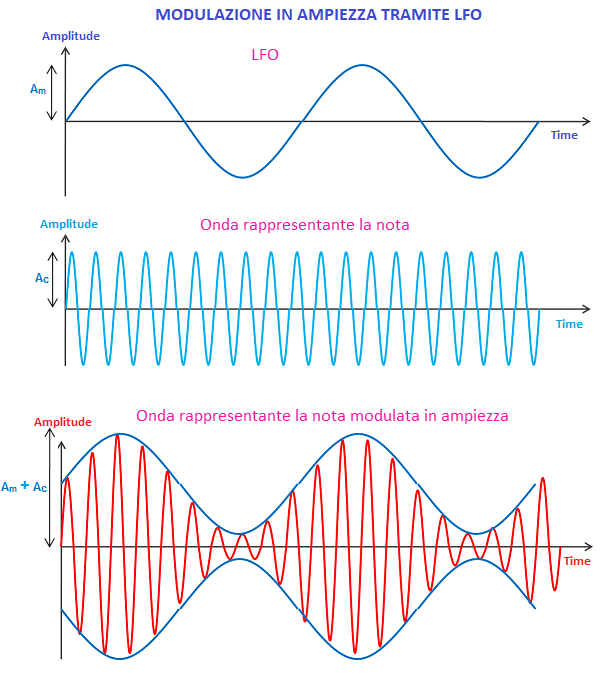
\includegraphics[width=\linewidth]{img/lfo.png}
    \caption{Un esempio di modulazione di ampiezza \cite{lfo_img}. I testi dell'immagine sono stati modificati per adattarli al contesto.}
    \label{fig:lfo}
\end{figure}
\subsubsection{Enveloper}
La sintesi audio porta con sè diversi problemi e complicazioni, la più comune tra queste è la presenza di un suono simile ad un “pop” durante la riproduzione.
Questi suoni sgradevoli sono causati suonando onde discontinue: quando lo speaker che riproduce l'audio, passando da una nota all'altra, percorre distanze troppo grandi in un tempo troppo breve.
Per evitare questo problema, ho utilizzato un Enveloper: un filtro che permette di gestire il volume in modo graduale.
L'enveloper è stato introdotto dall'ingegnere Robert Moog nel 1964, data la necessità di articolare il volume in maniera differente dai soli stati on/off.
I primi prototipi sviluppati di questo filtro caricavano e scaricavano lentamente dei condensatori attenuando il volume di conseguenza \cite{enveloper}.
Ad oggi, ogni sintetizzatore hardware e software mette a disposizione gli enveloper, la formula più comune è ADSR (Figura \ref{fig:asdr}), questo filtro gestisce l'andamento del volume in quattro stadi:
\begin{itemize}
    \item \textbf{Attack}: fase di crescita del volume, quando la nota viene premuta;
    \item \textbf{Decay}: fase di diminuzione del volume, la nota è ancora premuta, ma il volume diminuisce;
    \item \textbf{Sustain}: fase di mantenimento del volume, la nota è ancora premuta, il volume rimane stabile;
    \item \textbf{Release}: fase di diminuzione del volume, la nota viene rilasciata, il volume diminuisce.  
\end{itemize}
Siccome nel processo di sonificazione non vengono premuti effettivamente dei tasti, ho deciso di rimuovere le fasi di decay e sustain;
lo scopo dell'enveloper è stato quello di evitare il suono sgradevole citato precedentemente, aumentando e diminuendo il volume ad inizio e fine di una nota.
\begin{figure}[H]
    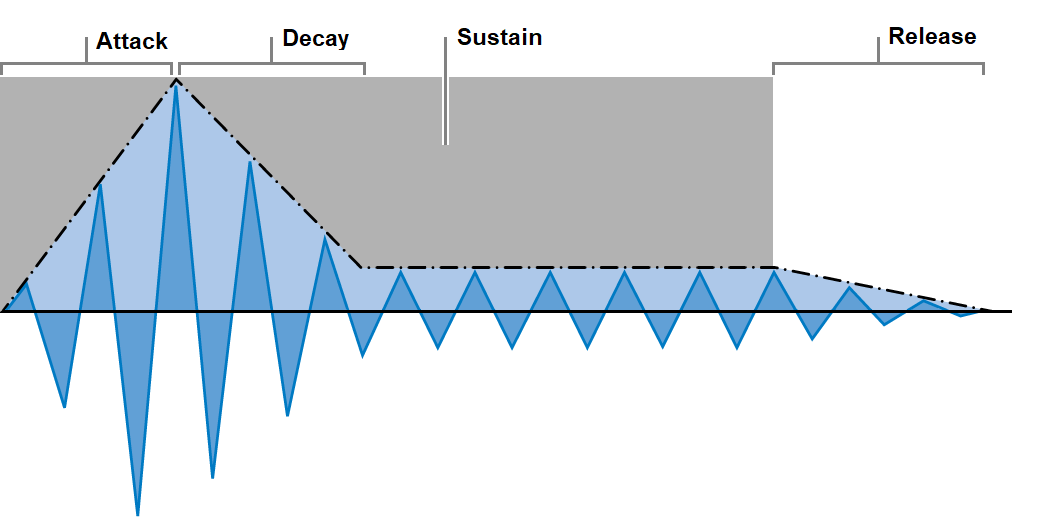
\includegraphics[width=\linewidth,scale=0.2]{img/adsr.PNG}
    \caption{Lo schema riassuntivo di un Enveloper ADSR \cite{env_img}.}
    \label{fig:asdr}
\end{figure}

\subsection{Creazione del video}
Per la generazione dell'animazione ho utilizzato matplotlib, una libreria di Data Visualization che permette di creare grafici.
In particolare, tramite \texttt{FuncAnimation} è possibile creare un'animazione a partire da una funzione che restituisce un grafico;
ogni rilevazione viene rappresentata da un frame, i quali vengono poi uniti in un unico file .gif ad intervalli di 0.5 secondi ciascuno.

\subsection{Unire Audio e Video}
L'aggiunta della traccia audio al file di animazione è stata possibile grazie a moviepy.
Moviepy è una libreria python per la manipolazione di video di diversi formati.
Per la funzionalità che ho utilizzato, moviepy richiama ffmpeg: una suite software cross platform per creare, tagliare, unire video.

\subsection{Altri software e hardware utilizzati}
\subsubsection{Ableton Live 10 Lite}
Ableton è una Digital Audio Workstation (DAW) che permette di registrare, modificare e riprodurre audio.
Ho utilizzato questo software in fase di prototipazione per comporre dei possibili risultati della sonificazione, applicare loro degli strumenti General MIDI e degli effetti audio.
Per la selezione delle note, ho utilizzato una tastiera compatibile con lo standard MIDI.
Durante la fase di testing, ho inoltre utilizzato Ableton per importare le traccie MIDI e gli audio sonificati, al fine di verificarne la correttezza.
\subsubsection{Audacity}
Audacity è un software open source per la manipolazione dell'audio.
Ho utilizzato questo software per analizzare in maniera più approfondita i campioni in fase di testing al fine di scoprire l'origine dei suoni sgradevoli.
Grazie alle funzione di zoom messa a disposizione è stato possibile individuare il problema con molta facilità.
\subsubsection{Visual Studio Code}
Visual Studio Code è un editor di testo open source, sviluppato da Microsoft.
Ho prediletto questo software per la sua semplicità di gestione di molteplici file simultaneamente, e per la sua completezza nelle funzionalità.
\subsubsection{Insomnia}
Insomnia è un software open source tramite il quale è possibile effettuare richieste HTTP e visualizzarne le risposte.
Ho utilizzato questo client in fase di test per comprendere la struttura delle risposte alle varie chiamate API effettuate.

\newpage
\section{Architettura del sistema schematizzata}
In Figura \ref{fig:uml} viene presentata una schematizzazione dell'architettura del sistema.
\begin{figure}[H]
    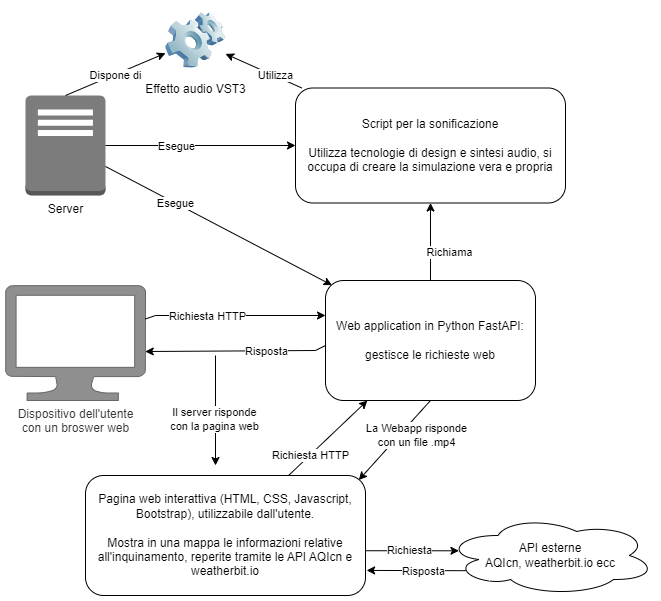
\includegraphics[width=\linewidth]{img/uml.png}
    \caption{L'Architettura del sistema.}
    \label{fig:uml}
\end{figure}